% !TEX root = ../diary-book.tex

\section{令和6年12月18日 シャワー測定頻度の推定}

\subsection{一次宇宙線到来頻度の推定}
2024-12-18 08:55:35

一次宇宙線の到来頻度について、推定を行うためにwikipedia \href{https://ja.wikipedia.org/wiki/%E5%AE%87%E5%AE%99%E7%B7%9A}{宇宙線} のページにある図を使った。

\begin{figure}[H]
   \centering
   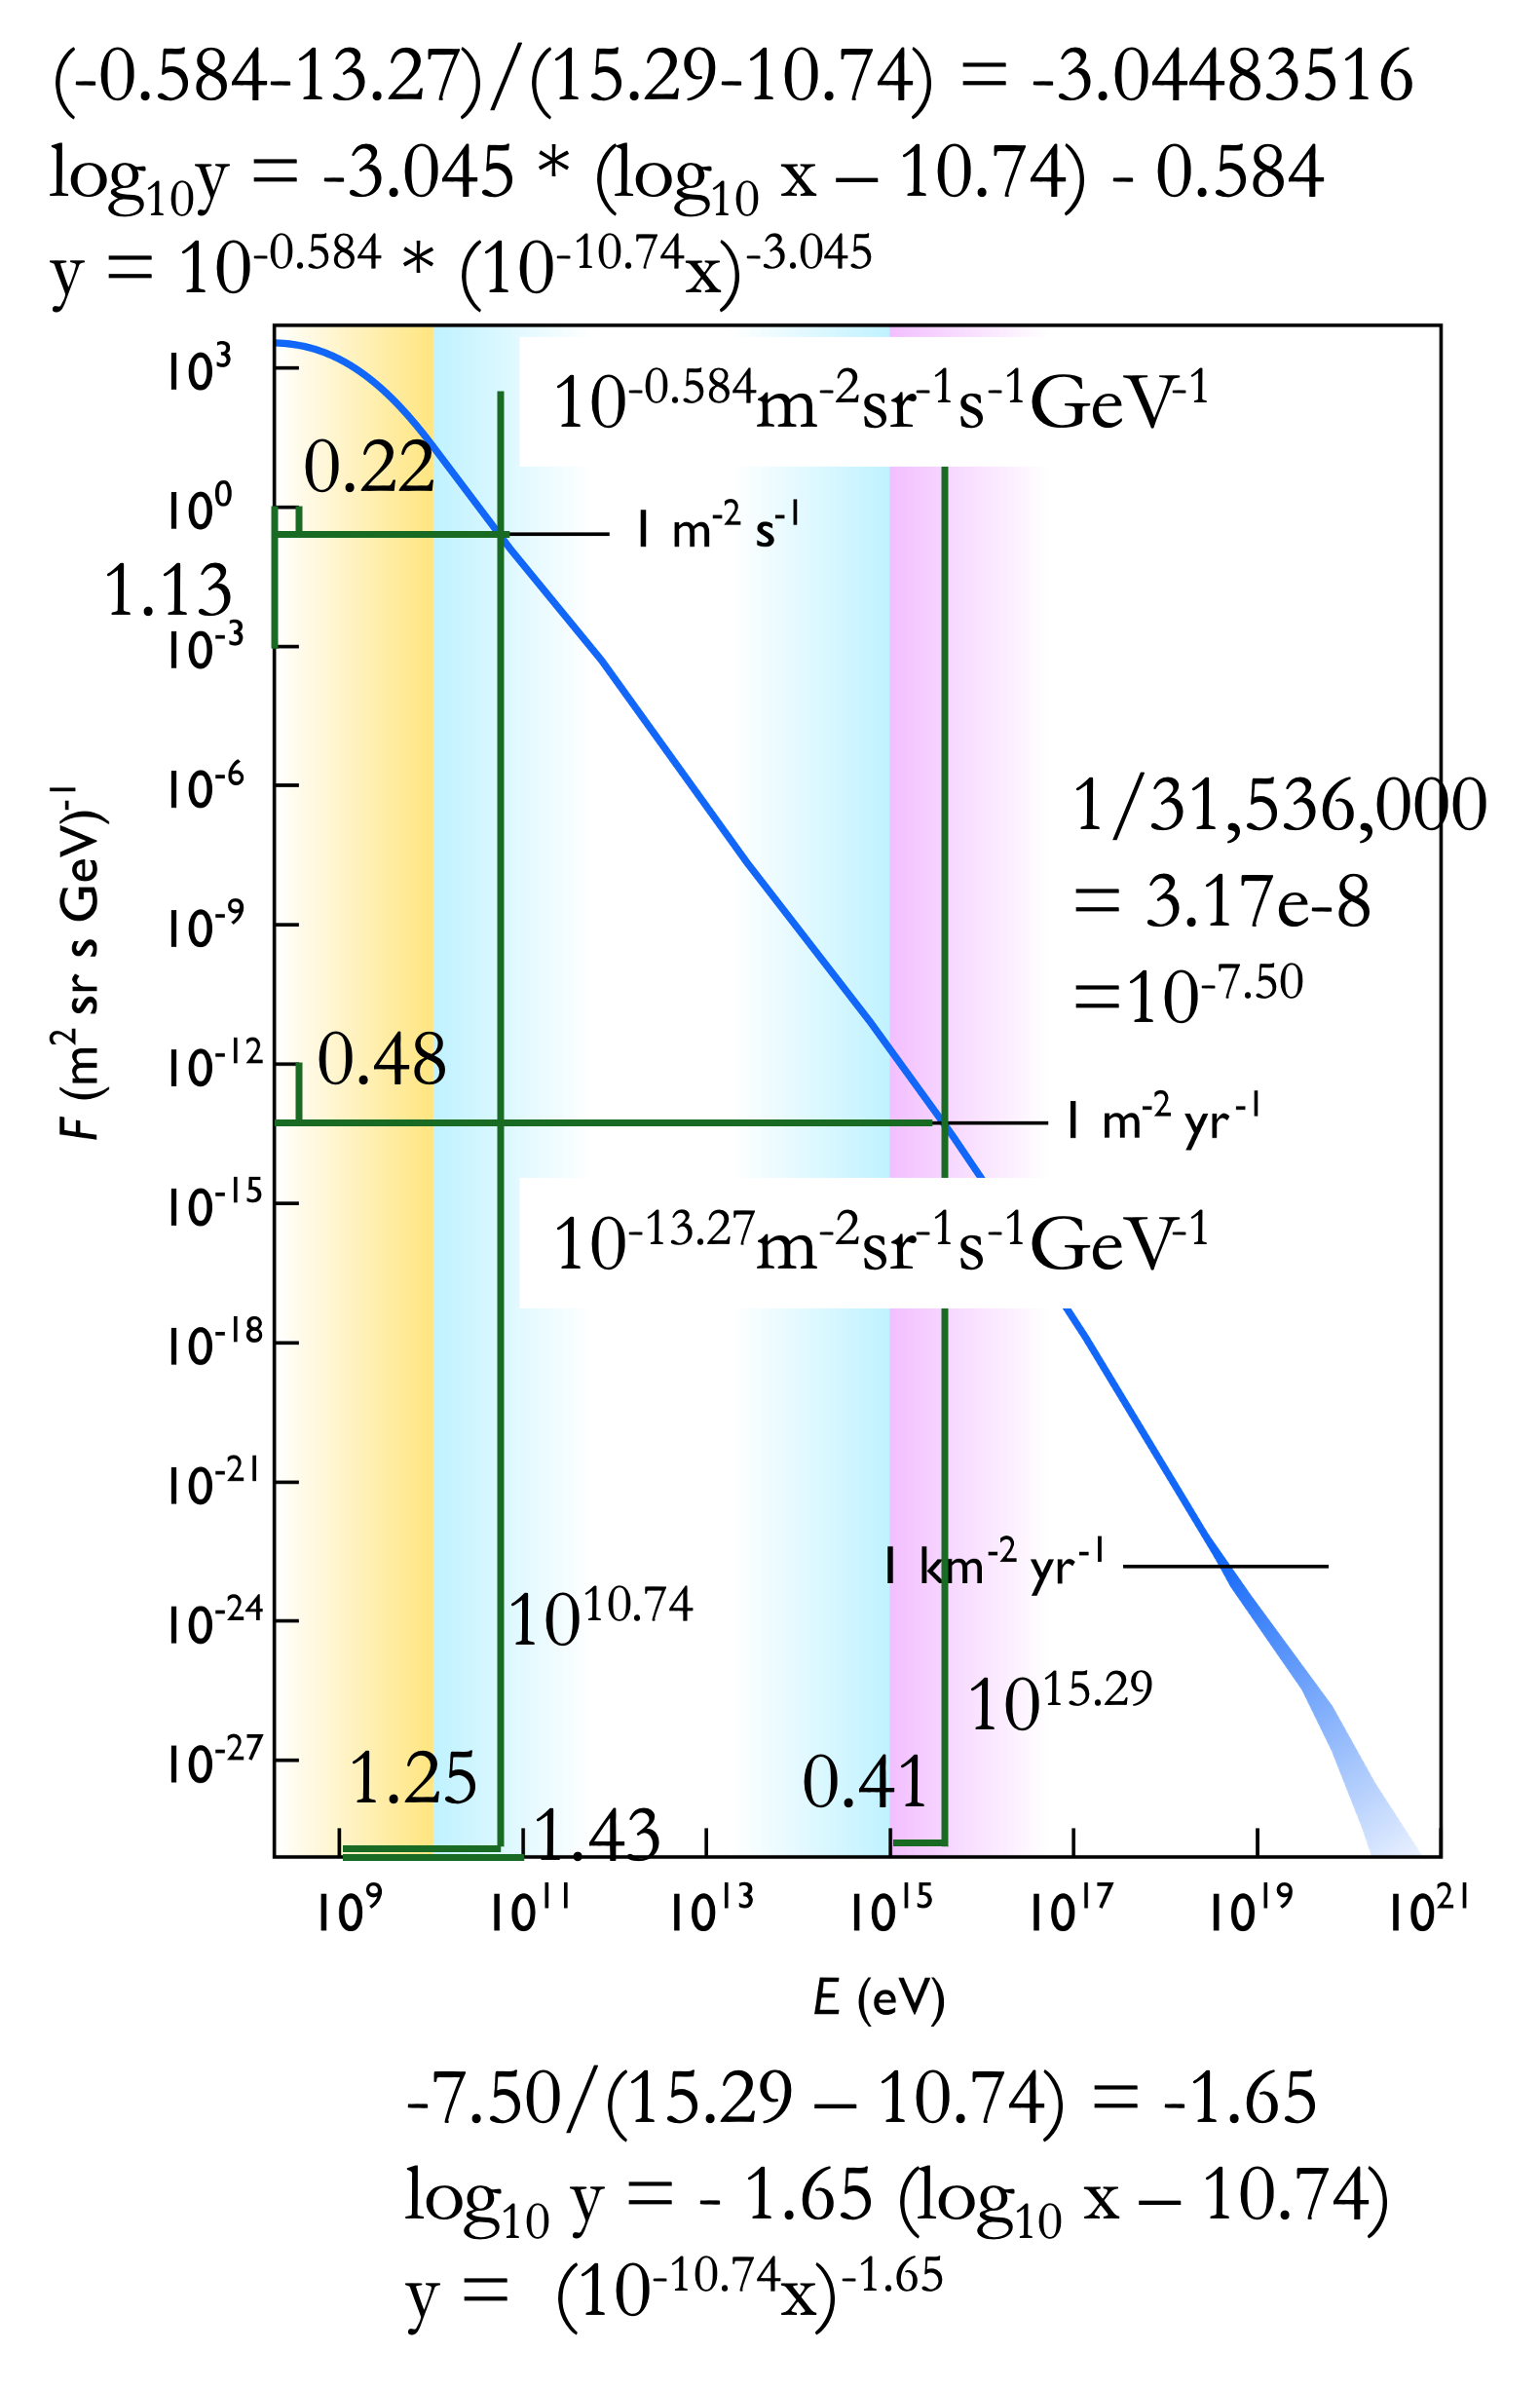
\includegraphics[width=.5\linewidth]{../../figs/ShowerRate/CosmicRayRateEstimation.png}
   \caption{宇宙線到来頻度の推定}
\end{figure}

\begin{equation}
   N = (10^{-10.74}x)^{-1.65}
\end{equation}

という式がえられて、これを使って角度積分した到来頻度を図\ref{fig:ShowerRate:IntegralRate}、フラックスそのものを\ref{fig:ShowerRate:IntegralFlux}に示す。
(2024-12-21 15:47:27 訂正、フラックスは正しいが到来頻度は積分している領域が異なるので、注意が必要。1~GeV 付近では 1~GeVビンで、1~PeV付近は 1~PeVビンで積分しているようにみえる。フラックスを積分していくほうが正しいか。)

\begin{figure}[H]
   \begin{minipage}[b]{.48\linewidth}
      \centering
      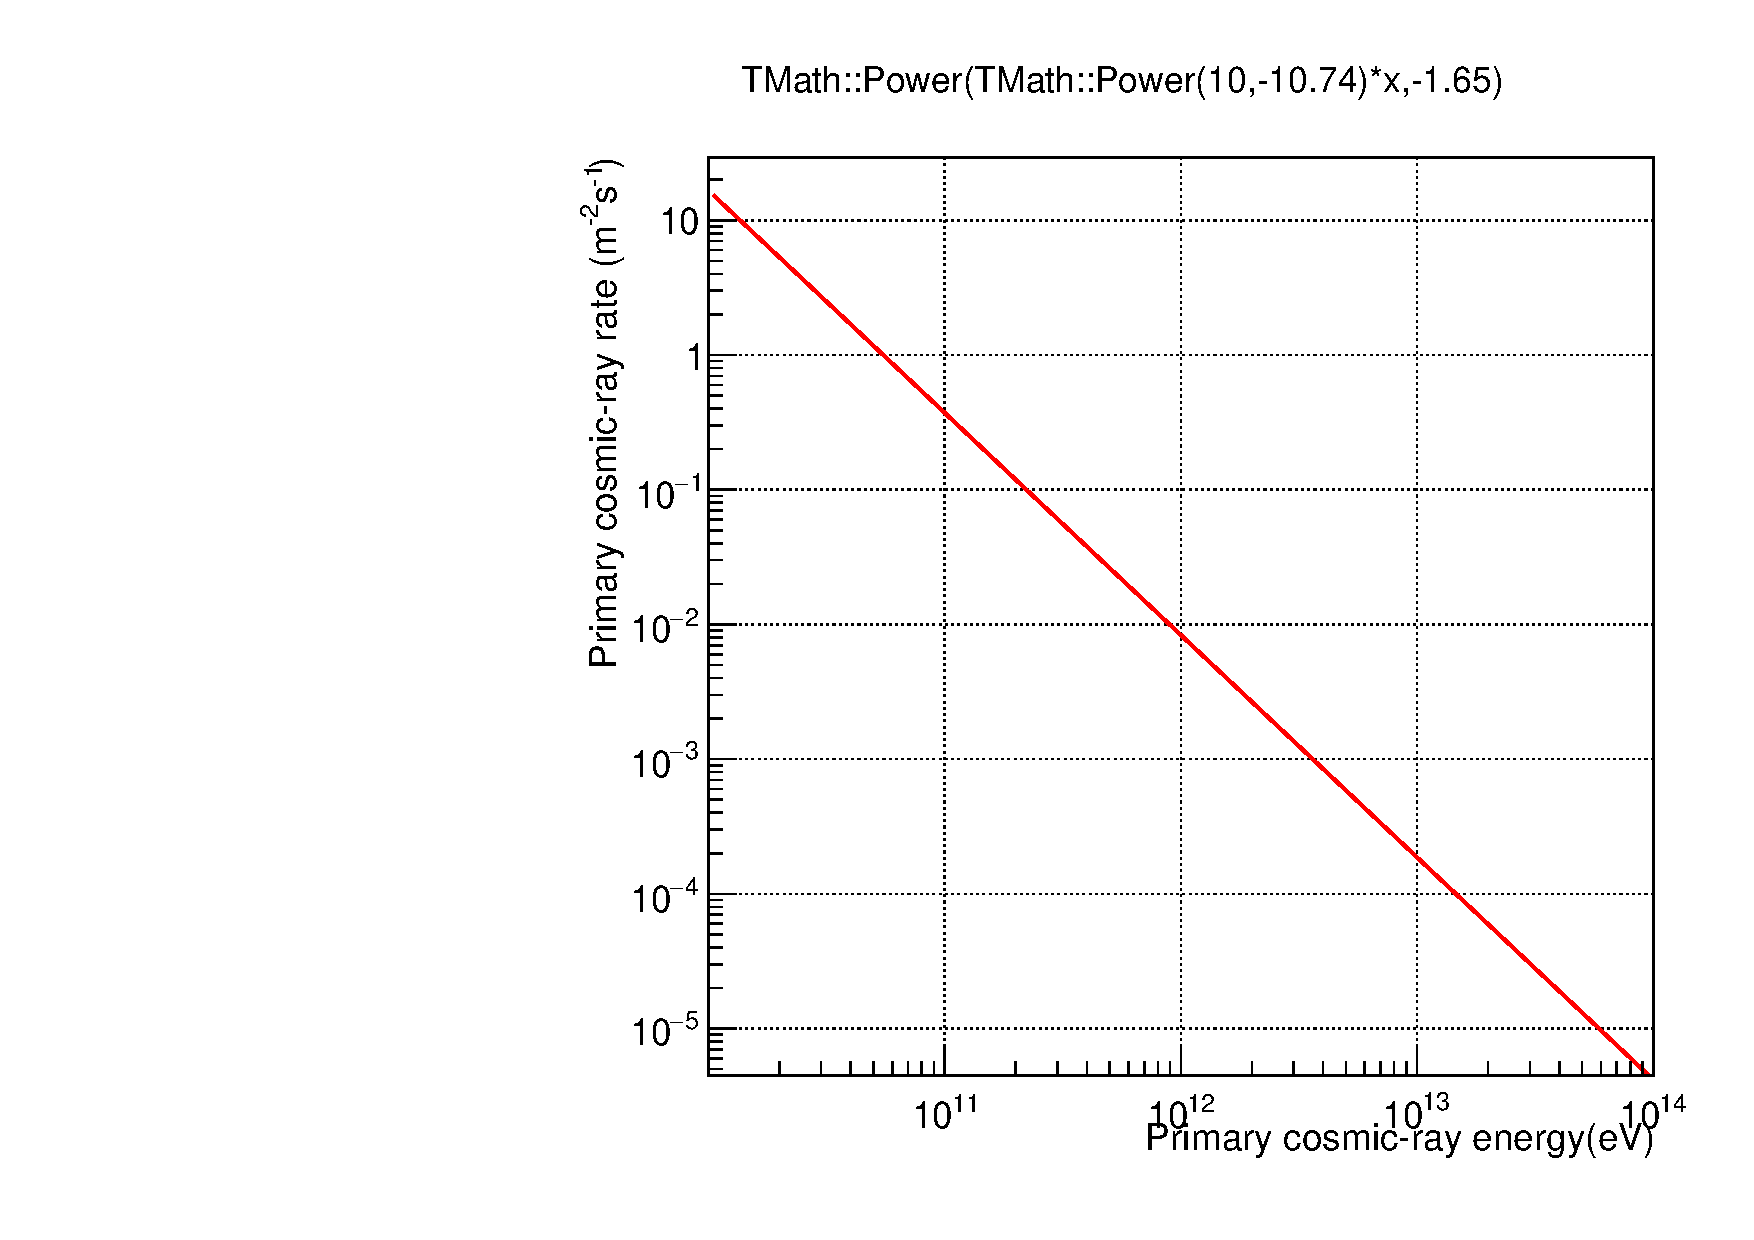
\includegraphics[width=.95\linewidth]{../../figs/ShowerRate/CosmicRayRate.pdf}
      \caption{角度積分した宇宙線到来頻度}\label{fig:ShowerRate:IntegralRate}
   \end{minipage}
   \begin{minipage}[b]{.48\linewidth}
      \centering
      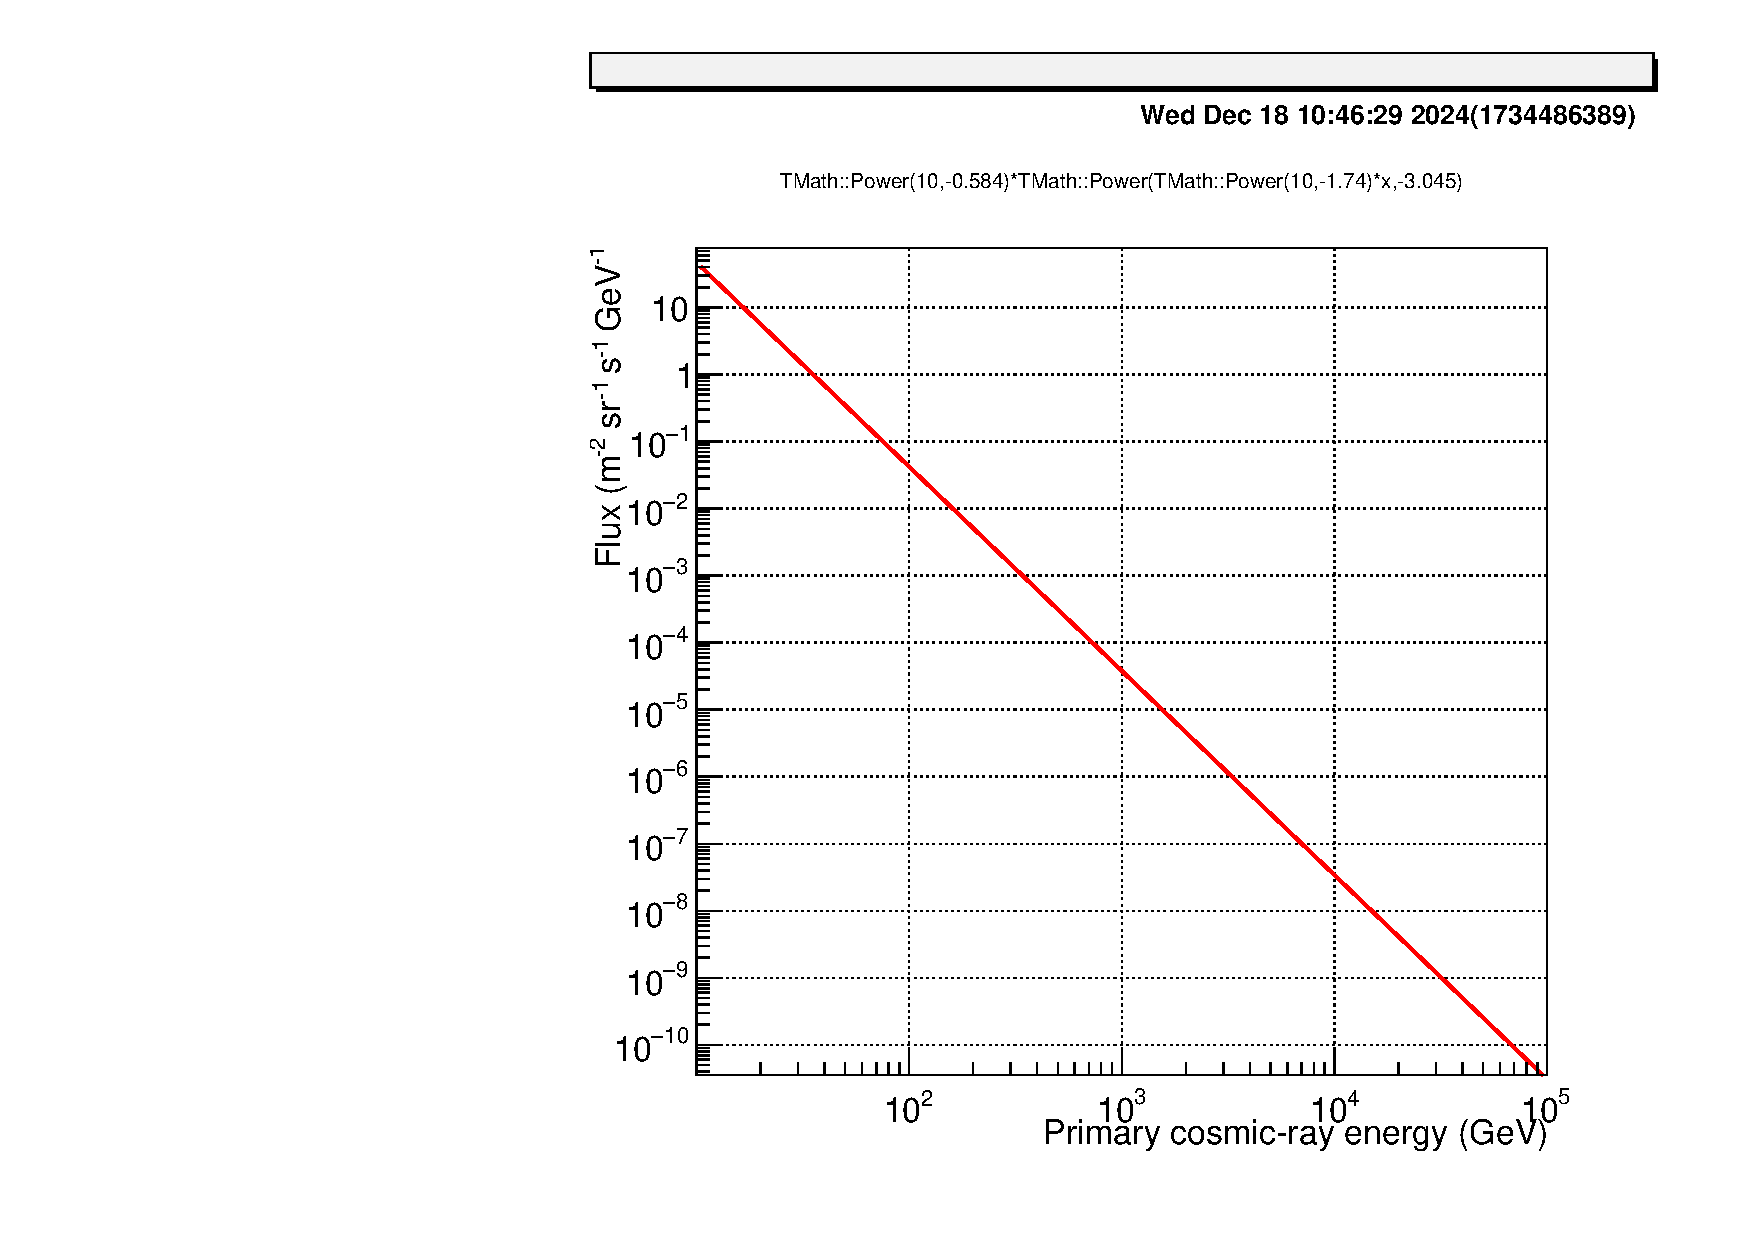
\includegraphics[width=.95\linewidth]{../../figs/ata03/figs/20241218/1734486389.pdf}
      \caption{宇宙線フラックス}\label{fig:ShowerRate:IntegralFlux}
   \end{minipage}
\end{figure}

典型的なエネルギーについて到来頻度を表\ref{tab:ShowerRate:IntegralRate}にまとめる。

\begin{table}
   \centering
   \caption{角度積分した宇宙線到来頻度}\label{tab:ShowerRate:IntegralRate}
   \begin{tabular}[H]{SS}
      \hline \hline
      {Energy} & {Rate} \\
      {(TeV)} & {(m$^{-2}$s$^{-1}$)} \\
      \hline
      1   & 8.3e-3 \\
      3 & 1.4e-3 \\
      10 & 1.9e-4 \\
      30 & 3.0e-5 \\
      100 & 4.2e-6 \\
      \hline
      \hline
   \end{tabular}
\end{table}

30~TeV程度のエネルギーになると100m四方でも1秒間に0.3回程度であってそれほど多くないことがわかる。ミューオンは手のひらに1秒間に一回程度到来しているのになぁ。。。低エネルギーの一次宇宙線からの寄与が大きいということが原因なのか？



\begin{figure}
   \centering
   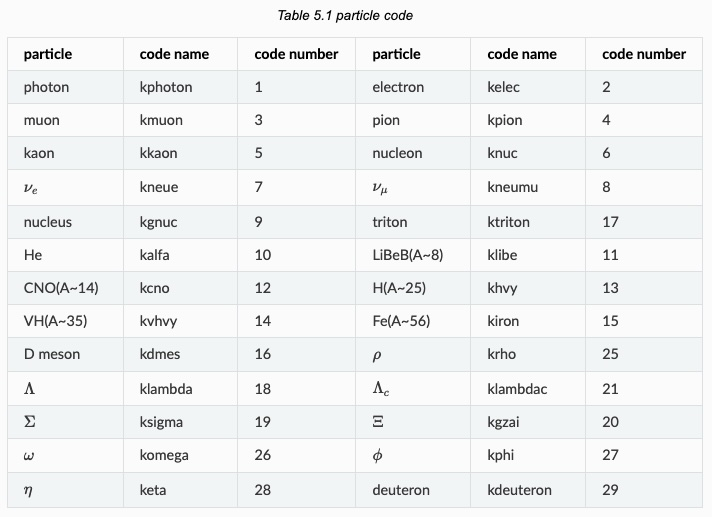
\includegraphics[width=.8\linewidth]{../../figs/COSMOS/ParticleCode.jpg}
   \caption{COSMOSでの粒子コードの定義}\label{fig:COSMOS:ParticleCode}
\end{figure}

一次宇宙線のエネルギーごとに粒子の検出効率を見積もれば、シャワー面をどのくらい同定可能化がわかる。正直なところ不安しかない。。。
10 TeV の宇宙線で 100 m四方の領域に、平均 4000 個の光子が地上に届いており、10 m 間隔においた 1m四方の検出器ではその 100分の1の粒子を捉えることができる。40 個。検出効率 10\% でも4個しか取ることができない。これではシャワー面を決めるだけで精一杯。。。ここにミューオンの計数率が入ってくる。